\section{Overview}
\begin{itemize}
    \item What is inheritance and why is it useful?
    \item Terminology and notation.
    \item Inheritance vs. composition.
    \item Deriving classes form existing classes.
        \begin{itemize}
            \item 3 types of inheritance.
        \end{itemize}
    \item Protected members and class access.
    \item Constructors and destructors.
        \begin{itemize}
            \item Passing arguments to base class constructors.
            \item Order of constructor and destructor calls.
        \end{itemize}
    \item Redefining base class methods.
    \item Class hierarchies.
    \item Multiple inheritance.
\end{itemize}

%%%%%%%%%%%%%%%%%%%%%%%%%%%%%%%%%%%%%%%%%%%%%%%%%%%%%%
\section{What is inheritance?}
\begin{itemize}
    \item What is it and why is it used?
        \begin{itemize}
            \item Provides a method for creating new classes from exiting classes.
            \item The new class contains the data and behaviurs of the existing class.
            \item Allow for reuse of existing classes.
            \item Allows us to fucus on the common attributes among a set of classes.
            \item Allws new classes to modify behaviors of existing classes to make it unique:
                \begin{itemize}
                    \item Without actually modifying the original class.
                \end{itemize}
            
            \item The object that is being inherited from must bear some relation to the inherited object. It does not make sense to inherit the object employee to the object planet. 
        \end{itemize}
    
    \item Related classes:
        \begin{itemize}
            \item Player: Enemy, Level boss, Hero, Super player, etcetera.
            \item Account: Savings account, checking account, trust account, etcetera.
            \item Shape: line, oval, circle, square, etcetera.
            \item Person: employee, student, faculty, staff, administrator, etcetera.
        \end{itemize}
    
    \item Sometimes the relationship between classes are clear and some may not. But their relationship must make sense.
    \item An example:
        \begin{itemize}
            \item Account is a parent class: balance, deposit, withdraw.
            \item Savings account inherits from Account: but needs to consider the interest rate.
            \item Checking account inherits from Account: but needs to have a minimum balance and a per check fee.
            \item Trust account inherits from Account: but it needs an interest rate.
        \end{itemize}
    
    \item Without inheritance code tends to duplicate, see the following implementation without inheritance:
        \begin{minted}[autogobble]{cpp}
            class Account {
                int balance, deposit, withdraw;
            };
            class Savings_Account {
                int balance, deposit, withdraw, interest rate;
            };
            class Checking_Account {
                int balance, deposit, withdraw, minimum_balance, per_check_fee;
            };
            class Trust_Account {
                int balance, deposit, withdraw, interest_rate;
            };
        \end{minted}
    
    
    \item With inheritance we can implemented like this:
        \begin{minted}[autogobble]{cpp}
            class Account {
                int balance, deposit, withdraw;
            };
            class Savings_Account : public Account {
                int interest_rate;
            };
            class Checking_Account : public Account {
                int minimum_balance, per_check_fee;
            };
            class Trust_Account : public Account {
                int interest_rate;
            };
        \end{minted}
\end{itemize}

%%%%%%%%%%%%%%%%%%%%%%%%%%%%%%%%%%%%%%%%%%%%%%%%%%%%%%
\section{Terminology and notation}
\begin{itemize}
    \item Inheritance:
        \begin{itemize}
            \item Process of creating new classes from existing classes.
            \item It is a reuse mechanism.
        \end{itemize}
    
    \item Single inheritance:
        \begin{itemize}
            \item A new class is created from another 'single' class.
        \end{itemize}
    
    \item Multiple inheritance:
        \begin{itemize}
            \item A new class is created from two or more other classes.
        \end{itemize}
\end{itemize}

\subsection{Terminology}
\begin{itemize}
    \item The base class is the parent class, or the super class:
        \begin{itemize}
            \item The class being extended or inherited from.
        \end{itemize}

    \item The derived class or child class, sub class:
        \begin{itemize}
            \item The class being created from the base class.
            \item Will inherit attributes and operations from base classes.
        \end{itemize}

    \item In UML we model class inheritance like this:
        \begin{figure}[H]
            \centering
            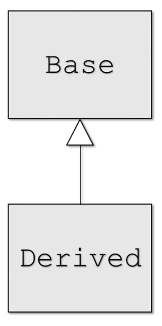
\includegraphics[width=\width\textwidth]{./figs/20220604170622.png}
            \caption{UML inheritance diagram}
        \end{figure}

    \item ´´Is-A'' relationship:
        \begin{itemize}
            \item Public inheritance.
            \item Derived classes are sub-types of their base classes.
            \item Can use a derived class object wherever we use a base class object.
        \end{itemize}
    
    \item Generalization:
        \begin{itemize}
            \item Combining similar classes into a single, more general class based on common attributes.
        \end{itemize}
    
    \item Specialization:
        \begin{itemize}
            \item Creating new classes from existing classes proving more speialized attributes or operations.
        \end{itemize}
    
    \item Inheritance or class hierarchies:
        \begin{itemize}
            \item Organization of our inheritance relationships.
        \end{itemize}
\end{itemize}

\subsection{Inhertiance}
\begin{itemize}
    \item Class hierarchy denote the order in which the attributes will be shared. The further up we go in the hierarchy we become more general and the further down we become more specialized:
        \begin{itemize}
            \item A
            \item B is derived from A
            \item C is derived from A
            \item D is derived from C
            \item E is derived from D
        \end{itemize}
        \begin{figure}[H]
            \centering
            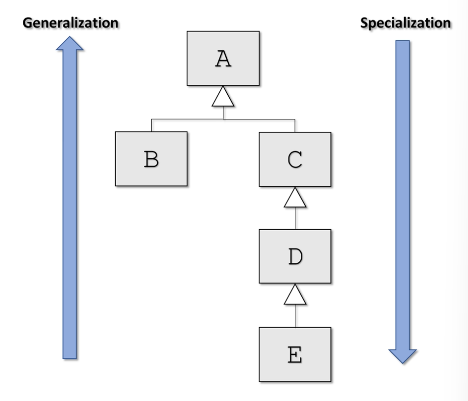
\includegraphics[width=\width\textwidth]{./figs/20220604225629.png}
            \caption{Inheritance hierarchy}
        \end{figure}
    
    \item Another example:
        \begin{itemize}
            \item Person 
            \item Employee is derived from Person
            \item Student is derived from Person
            \item Faculty is derived from Employee 
            \item Staff is derived from Employee 
            \item Administrator is derived from Employee
        \end{itemize}
        \begin{figure}[H]
            \centering
            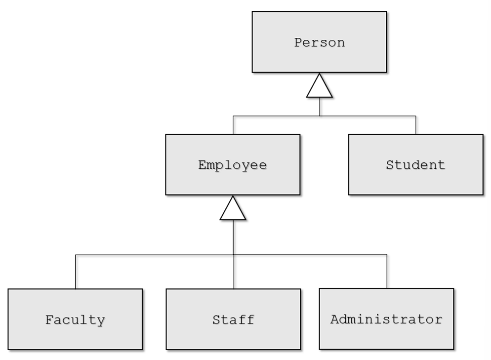
\includegraphics[width=\width\textwidth]{./figs/20220604225820.png}
            \caption{}
        \end{figure}
\end{itemize}

%%%%%%%%%%%%%%%%%%%%%%%%%%%%%%%%%%%%%%%%%%%%%%%%%%%%%%
\section{Inheritance vs composition}
\begin{itemize}
    \item Until now we have seen public inheritance.
    \item Public inheritance: 
        \begin{itemize}
            \item Create an ´´Is-A'' relationship.
                \begin{itemize}
                    \item Employee 'is-a' Person.
                    \item Checking Account 'is-a' Account.
                    \item Circle 'is-a' Shape.
                \end{itemize}
        \end{itemize}
    
    \item Composition:
        \begin{itemize}
            \item Creates a 'has-a' relationship.
                \begin{itemize}
                    \item Person 'has-a' Account.
                    \item Player 'has-a' Special Attack.
                    \item Circle 'has-a' Location.
                \end{itemize}
        \end{itemize}
\end{itemize}

\subsection{Example}
\begin{figure}[H]
    \centering
    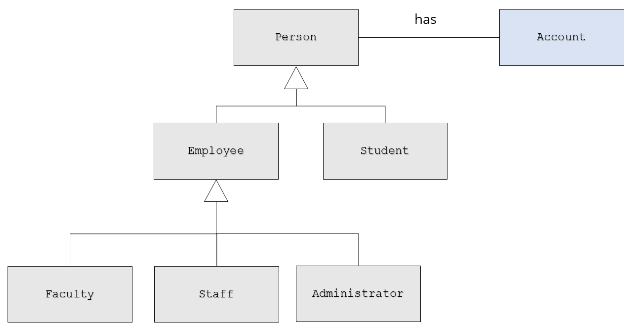
\includegraphics[width=\width\textwidth]{./figs/20220604230251.png}
    \caption{Example of composition}
\end{figure}
\begin{itemize}
    \item Account does not have an 'is-a' relationship with Person, it has a 'has-a' relation.
    \item We create the association at Person since this means all subclasses that inherit Person will also have the Account relationship.
    \item Class members have an 'has-a' relationship with the class being declared.
        \begin{figure}[H]
            \centering
            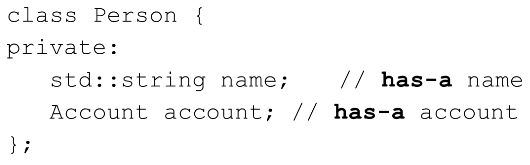
\includegraphics[width=\width\textwidth]{./figs/20220604230548.png}
            \caption{'has-a' relation between data members and class}
        \end{figure}
\end{itemize}

%%%%%%%%%%%%%%%%%%%%%%%%%%%%%%%%%%%%%%%%%%%%%%%%%%%%%%
\section{Deriving  classes from existing classes}
\begin{itemize}
    \item The syntax for the base class:
        \begin{minted}[autogobble]{cpp}
            class Base {
                // Base class members ...
            };
            class Derived : <access-specifier> Base {
                // Derived class members ...
            };
        \end{minted}
        \begin{itemize}
            \item The $\displaystyle \langle \texttt{access-specier} \rangle$ can be: public, private, or protected.
        \end{itemize}
    
    \item Types of inheritance:
        \begin{itemize}
            \item Public: 
                \begin{itemize}
                    \item Most common.
                    \item Establishes an 'is-a' relationship between derived and base classes.
                \end{itemize}
            
            \item Private and protected:
                \begin{itemize}
                    \item Establishes ´´derived class has a base class'' relationship.
                    \item ´´Is implemented in terms of'' relationship.
                    \item Different from composition.
                    \item Private and protected inheritance are beyond the scope of this course.
                \end{itemize}
        \end{itemize}
    
    \item Example:
        \begin{minted}[autogobble]{cpp}
            class Account {
                // Account class members ...
            }; 
            class Savings_Account : public Account {
                // Savings_Account class members ...
            };
        \end{minted}
        \begin{itemize}
            \item Savings\_Account 'is-a' Account.
        \end{itemize}
        \begin{minted}[autogobble]{cpp}
            Account account {};
            Account *p_account = new Account();
            account.deposit(1000.0);
            p_account->withdraw(200.0);
            delete p_account;
        \end{minted}
        \begin{minted}[autogobble]{cpp}
            Savings_Account sav_account {};
            Savings_Account *p_sav_account = new Savings_Account();
            sav_account.deposit(1000.0);
            p_sav_account->withdraw(200.0);
            delete p_sav_account;
        \end{minted}
\end{itemize}

%%%%%%%%%%%%%%%%%%%%%%%%%%%%%%%%%%%%%%%%%%%%%%%%%%%%%%
\section{Protected emers and class access}
\begin{itemize}
    \item The protected class member modifier:
        \begin{minted}[autogobble]{cpp}
            class Base {
                protected: 
                    // protected class members ...
            };
        \end{minted}
    
    \item Give the following properties:
        \begin{itemize}
            \item Protected class members are accessible from the base class itself.
            \item Protected class members are accessible from classes derived from base.
            \item Protected class members are not accessible by objects of base or derived.
        \end{itemize}
    
    \item C++ handles 3 types of inheritance: public, protected and private.
\end{itemize}

\subsection{Public inheritance}
\begin{itemize}
    \item When inheriting public class members the base class will inherit the class members are public also, and the inherited class will also have access to the base class members.
    \item It does not matter how deep the class hierarchy goes the attributes will be accesable by all derived classes.
\end{itemize}
\begin{figure}[H]
    \centering
    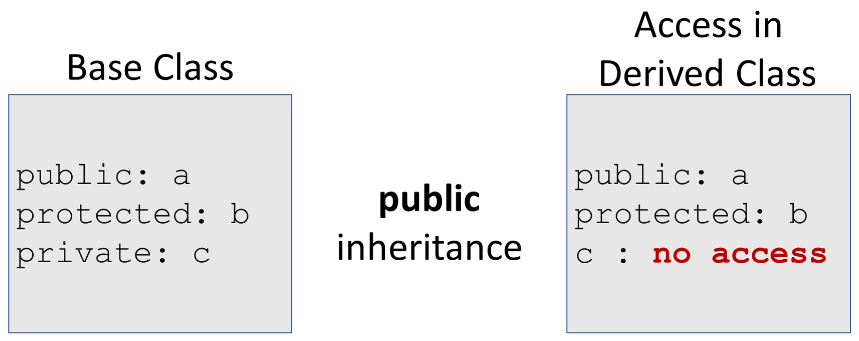
\includegraphics[width=\width\textwidth]{./figs/20220614163228.png}
    %\caption{}
\end{figure}

\subsection{Protected inheritance}
\begin{itemize}
    \item When inherting protected class members the derived class will inherit them as protected also, and will have access to them.
    \item Protected is not 'is-a' inhertiance.
    \item When inheriting using protected inheritance public attributes are inhertied as protected. Protected attributes are inherited as protected and private attributes are inaccessible.
\end{itemize}
\begin{figure}[H]
    \centering
    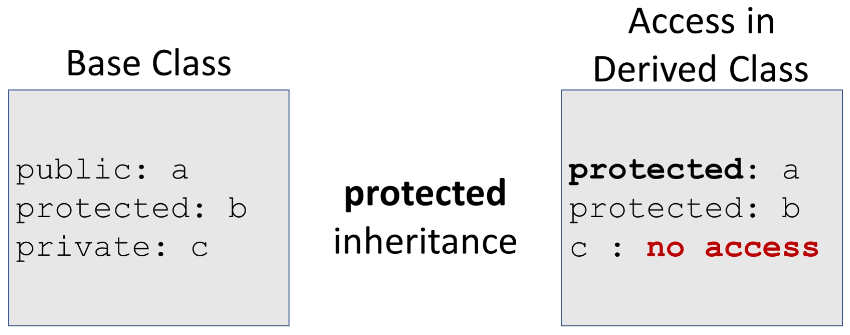
\includegraphics[width=\width\textwidth]{./figs/20220614163610.png}
    %\caption{}
\end{figure}


\subsection{Private inheritance}
\begin{itemize}
    \item When inheriting private class members the derived class will inherit them but will not be able to modify them, the derived class will have no access. Any attempt to modify or use them in any way will result in a compiler error.
    \item Private inheritance is not 'is-a' inheritance.
    \item When inherting using private, all public and protected attributes are inherited as private, the base class private attributes are inaccessible to the derived class.
\end{itemize}
\begin{figure}[H]
    \centering
    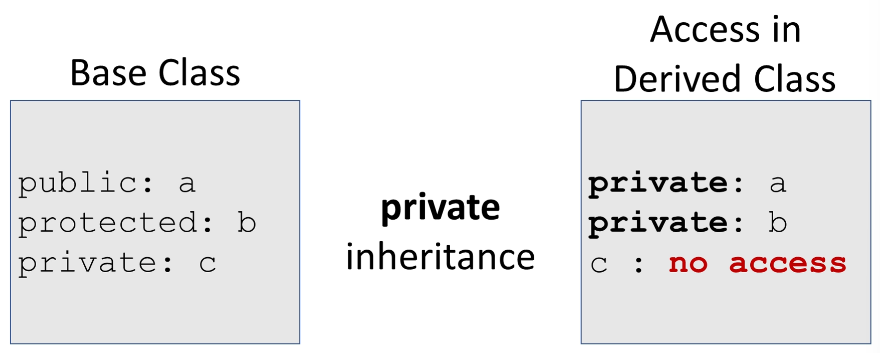
\includegraphics[width=\width\textwidth]{./figs/20220614163719.png}
    %\caption{}
\end{figure}

\subsection{Friends of base classes}
\begin{itemize}
    \item Remember that if a class is a friend of a base class then they will have access to public, private and protected information in this class.
\end{itemize}

\subsection{Example}
\begin{minted}[autogobble]{cpp}
    #include <iostream>
    using namespace std;

    class Base {
        public: 
            int a {0};
            void display() {cout << a << ", " << b << c << endl;} // public method.
        protected:
            int b {0};
        private:
            int c {0};
    };

    class Derived : public Base {
        public:
        // a will be public, accessible.
        // b will be protected, accessible.
        // c inherited but will not be accessible.
        void access_base_members() {
            a = 100; // OK
            b = 200; // OK
            // c = 300; // not accessible, compiler error.
        }   
    };

    int main() {
        Base base;
        base.a = 100; // a is public, OK.
        // base.b = 200; // b is protected, compiler error.
        // base.c = 300; // c is private, compiler error.
        Derived derived;
        derived.a = 100; // OK
        // derived.b = 200; // Error, protected.
        // derived.c = 300; // Error, private.
        return (0);
    }
\end{minted}

%%%%%%%%%%%%%%%%%%%%%%%%%%%%%%%%%%%%%%%%%%%%%%%%%%%%%%
\section{Constructors and destructors}
\begin{itemize}
    \item Constructors:
    \begin{itemize}
            \item A derived class inherits from its base class.
            \item The base part of the derived class MUST be initialized BEFORE the derived class is initialized.
            \item When a derived object is created:
                \begin{itemize}
                    \item Base class constructor executes then.
                    \item Derived class constructor executes.
                \end{itemize}
        \end{itemize}
    \item Destructors:
        \begin{itemize}
            \item Class destructors are invoked in the reverse order as constructors.
            \item The derived part of the derived class must be destroyed before the base class destructor is invoked.
            \item When a derived objet is destroyed:
                \begin{itemize}
                    \item Derived class destructor executes then
                    \item Base class destructor executes
                    \item Each destructor should free resources allocated in it's own constructors
                \end{itemize}
        \end{itemize}
    
    \item A derived class does not inherit the following:
        \begin{itemize}
            \item Base class constructors
            \item Base class destructor
            \item Base class overloaded assignment operators.
            \item Base class friends.
        \end{itemize}
    
    \item However, the derived class constructors, destructors, and overloaded assignment operators can invoke the base class versions.
    \item C++11 allows explicit inheritance of base 'non-special' constructors with:
        \begin{itemize}
            \item \mintinline{cpp}{using Base::Base;} anywhere in the derived class declaration.
            \item Lots of rules involed, often better to define constructors yourself. For example no move constructor is copied, there are a lot of rules.
        \end{itemize}
    
    \item Examples:
        \begin{minted}[autogobble]{cpp}
            #include <iostream>
            using namespace std;

            class Base {
                public:
                Base()  {cout << "Base constructor" << endl;}
                ~Base() {cout << "\tBase destructor" << endl;}
            };

            class Derived : public Base {
                public:
                Derived()  {cout << "Derived constructor" << endl;}
                ~Derived() {cout << "\tDerived destructor" << endl;}
            };

            int main() {
                {
                    Base b;
                }
                {
                    Derived d;
                }
            }
            /* Output:
            Base constructor
                    Base destructor
            Base constructor
            Derived constructor
                    Derived destructor
                    Base destructor
            */
        \end{minted}
\end{itemize}

%%%%%%%%%%%%%%%%%%%%%%%%%%%%%%%%%%%%%%%%%%%%%%%%%%%%%%
\section{Passing arguments to the base class constructors}
\begin{itemize}
    \item When you have several constructors being used in the base class, sometimes it is not clear which to use when instantiating the base class from the derived class. 
    \item The base part of the derived class must be initialized first.
    \item How can we control exactly which base class constructor is used during initialization?
    \item We can invoke the whichever base class constructor we wish to use in the initialization list of the derived class. 
    \item Example:
        \begin{minted}[autogobble]{cpp}
            class Base {
                Base();
                Base(int);
            };
            Derived::Derived(int x) : Base(x) /*optional initializers for derived*/ {
                // derived initializer code.
            }
        \end{minted}
    
    \item If we dont explicitly invoke the base class constructor then the base class constructor without args will be invoked automatically because the base class must be initialized before the derived class.
    \item Example:
        \begin{minted}[autogobble]{cpp}
            #include <iostream>
            using namespace std;

            class Base {
                int value;
            public:
                Base() : value{0} { cout << "Base no args constructor" << endl; }
                Base(int x) : value{x} {cout << "Int base constructor" << endl; }
            };

            class Derived : public Base {
                int doubled_value;
            public:
                Derived() : Base{}, doubled_value{0} { cout << "Derived no args constructor" << endl; }
                Derived(int x) : Base{x}, doubled_value{x*2} { cout << "int derived constructor" << endl; }
            };

            int main() {
                {
                    Base b1;
                    Base b2(3);
                }
                {
                    Derived d1;
                    Derived d2(4);
                }
            }
            /* Output:
            Base no args constructor
            Int base constructor
            Base no args constructor
            Derived no args constructor
            Int base constructor
            */
        \end{minted}
        \begin{figure}[H]
            \centering
            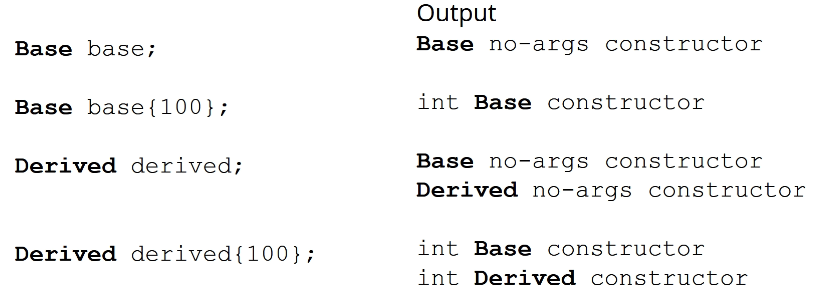
\includegraphics[width=\width\textwidth]{./figs/20220614231309.png}
            %\caption{}
        \end{figure}
\end{itemize}

%%%%%%%%%%%%%%%%%%%%%%%%%%%%%%%%%%%%%%%%%%%%%%%%%%%%%%
\section{Copy/move constructors and operator= with derived classes}
\begin{itemize}
    \item Copy/move onstructors are not inherited from the base class.
    \item You may not need to provide your own:
        \begin{itemize}
            \item Since the compiler can provide default versions and that might work just fine.
        \end{itemize}
    
    \item We can explicitly invke the base class versions from the derived class.
    \item We can invoke the base copoy constructor explicitly:
        \begin{itemize}
            \item Derived object 'other' will be sliced.
        \end{itemize}
        \begin{minted}[autogobble]{cpp}
            Derived::Derived(const Derived &other) 
                : Base(other) {
                    // code
                }
        \end{minted}
    
    \item Copy constructors:
        \begin{itemize}
            \item The base class:
                \begin{minted}[autogobble]{cpp}
                    class Base {
                        int value;
                    public:
                        // same constructors as previos example.
                        Base(const Base &other) 
                            : value{other.value} {
                            cout << "base copy constructor" << endl;
                        }
                    };
                \end{minted}
            
            \item The derived class:
                \begin{minted}[autogobble]{cpp}
                    class Derived : public Base {
                        int double_value;
                    public:
                        // same constructors as previos example
                        Derived(const Derived &other) 
                            : Base(other), doubled_value{other.double_value} 
                            {
                            cout << "derived copy constructor" << endl;
                        }
                    }
                \end{minted}
        \end{itemize}
    
    
    \item Operator=:
        \begin{itemize}
            \item Base class:
                \begin{minted}[autogobble]{cpp}
                    class Base {
                        int value;
                    public:
                        // same constructors as previos example.
                        Base &operator=(const Base &rhs) {
                            if (this != &rhs) {
                                value = rhs.value; // assign
                            }
                            return *this;
                        }
                    };
                \end{minted}
            
            \item Derived class:
                \begin{minted}[autogobble]{cpp}
                    class Derived : public Base {
                        int double_value;
                    public:
                        // same constructors as previos example
                        Derived &operator=(const Derived &rhs) {
                            if (this != &rhs) {
                                Base::operator=(rhs); // assign base part.
                                doubled_value = rhs.doubled_value; // assign derived part.
                            }
                            return *this;
                        }
                    }
                \end{minted}
        \end{itemize}
        
    \item Copy/move constructors and overloaded operator=:
        \begin{itemize}
            \item Often you do not need to provide your own.
            \item If you DO NOT define them in the derived class:
                \begin{itemize}
                    \item Then the compiler will create them automatically and call the base class's version.
                \end{itemize}
            
            \item If you DO provide derived versions:
                \begin{itemize}
                    \item Then you must invoke the base versions explicitly yourself.
                \end{itemize}

            \item Be careful with raw pointers:
                \begin{itemize}
                    \item Especially if base and derived each have raw pointers.
                    \item Provide them with deep copy semantics.
                \end{itemize}
        \end{itemize}
\end{itemize}

%%%%%%%%%%%%%%%%%%%%%%%%%%%%%%%%%%%%%%%%%%%%%%%%%%%%%%
\section{Redefining base class methods}
\begin{itemize}
    \item One of the most useful features of inheritance is that base class methods are available to the derived class.
    \item Derived class can directly invoke base class methods.
    \item Derived class can override or redefine base class methods.
    \item Very powerful in the conext of polymorphism (next section).
    \item To redefine a method in the derived class you just need to provide a method by the same name in the derived class.
    \item Example:
        \begin{minted}[autogobble]{cpp}
            class Account {
            public:
                void deposit(double amount) { balance += amount; }
            };

            class Savings_Account {
            public:
                void deposit(double amount) { // redefines base class methods.
                    amount += some_interest;
                    Account::deposit(amount); // invoke call base class method.
                }
            };
        \end{minted}
    
    \item Notice that this allows us to not repeat code, since we can make the modification to the amount and then call the base class method.
\end{itemize}

\subsection{Static binding of method calls}
\begin{itemize}
    \item Binding of which method to use is done at compile time:
        \begin{itemize}
            \item Default binding for C++ is static.
            \item Derived class objects will use Derived::deposit.
            \item But, we can explicitly invoke Base::deposit from Derived::deposit.
            \item OK, but limited -- much more powerful approach is dynamic binding which we will see in the next section.
        \end{itemize}
    
    \item Examples of static binding of method calls:
        \begin{minted}[autogobble]{cpp}
            Base b;
            b.deposit(1000.0); // Base::deposit
            
            Derived d;
            d.deposit(1000.0); // Derived::deposit

            Base *ptr = new Derived();
            ptr->deposit(1000.0); // Base:deposit, because it is apointer to a base class.
        \end{minted}
    
    \item By default C++ uses static binding. Which means that it determines the method to use at compile time.
\end{itemize}

%%%%%%%%%%%%%%%%%%%%%%%%%%%%%%%%%%%%%%%%%%%%%%%%%%%%%%
\section{Multiple inheritance}
\begin{itemize}
    \item A derived class inherits from two or more base classes at the same time.
    \item The base classes may belong to unrelated class hierarchies.
    \item A department chair:
        \begin{itemize}
            \item Is-a faculty and
            \item Is-a administrator
        \end{itemize}
        \begin{figure}[H]
            \centering
            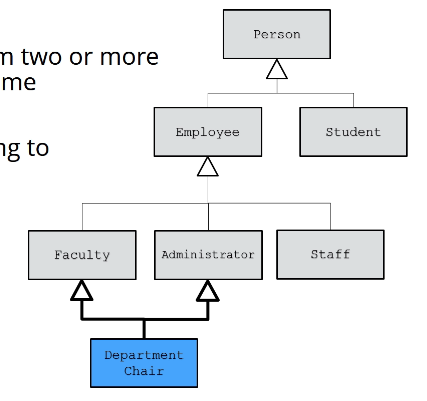
\includegraphics[width=\width\textwidth]{./figs/20220615221441.png}
            %\caption{}
        \end{figure}
    
    \item C++ syntax:
        \begin{minted}[autogobble]{cpp}
            class Department_Chair : public Faculty, public Administrator {
                ...
            };
        \end{minted}
        \begin{itemize}
            \item This feature is beyond the scope of this course.
            \item It has some compelling use-cases.
            \item Easily misused.
            \item Can be very complex.
            \item We can also use the other types of inheritance, not just public, you can use protected, private etcetera.
        \end{itemize}
\end{itemize}

\section{Section challenge}
